\section{Introduction}
Introduction

s\newpage

\section{State Of The Art - Privacy}
\label{section:Introduction}
To describe methods of CI with NodeJS

\subsection{First Section}

\begin{figure}[h!]
  \centering
      
\includegraphics[width=0.4\textwidth]{images/Perlin-Coherent.png}
  \caption{Just some example figure}
\end{figure}

\subsection{Next section}

\subsubsection{subsubsection}
 examplecite \cite{danezis2015privacy}

\subparagraph{subparagraph}
\footcite{hansen2012top}
\footcite{rost2009datenschutz}
\footcite{probst2012generische}

\begin{itemize}
  \item Itemlist 1
  \item Itemlist 2
\end{itemize} \cite{cranorplatform}

\section{Next Section}
\label{section:Label}

\textit{Texit Option}

\begin{figure}[h!]
  \centering
      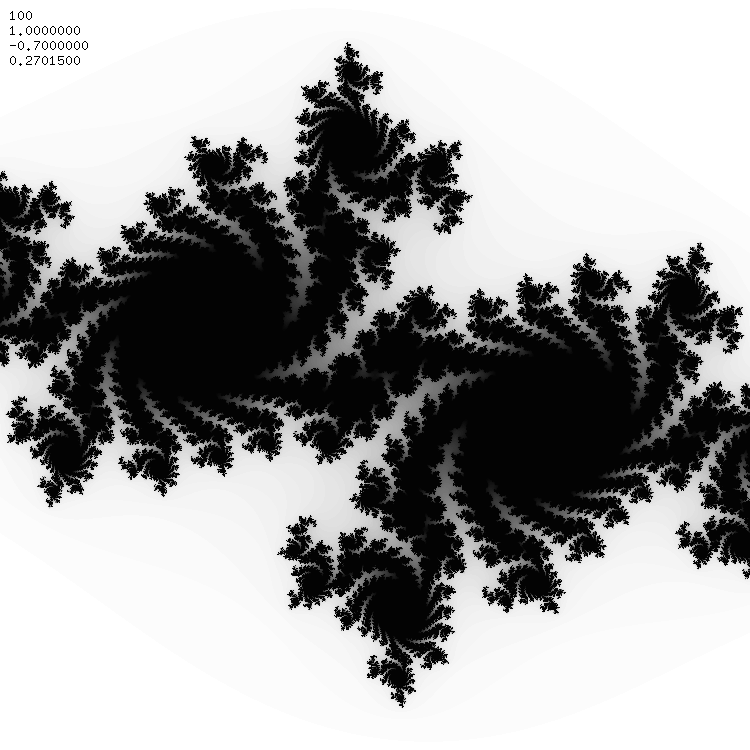
\includegraphics[width=0.2\textwidth]{images/Julia-Fractal.png}
  \caption{Exampelimage}
\end{figure}

\subparagraph{Unforgeability}
\label{subp:subparagraph_name}
Only a suitable service can produce a credential. A credential should not be forgeable by other sources, and should involve only attributes that are valid.

\begin{figure}[h!]
  \centering
      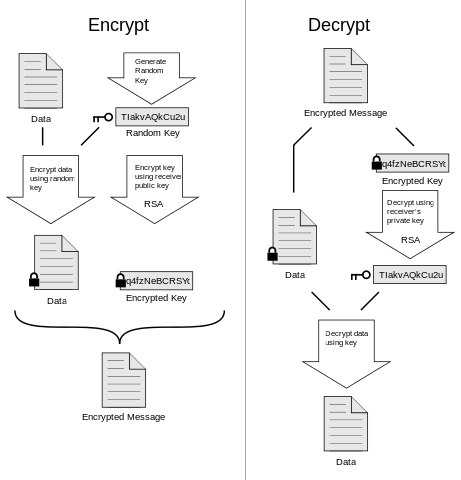
\includegraphics[width=0.5\textwidth]{images/pgp.png}
  \caption{PGP Encryption/Decryption}
\end{figure}

Graphic by \url{http://en.wikipedia.org/wiki/Pretty_Good_Privacy#/media/File:PGP_diagram.svg}
